\documentclass[english,floatsintext,man]{apa6}

\usepackage{amssymb,amsmath}
\usepackage{ifxetex,ifluatex}
\usepackage{fixltx2e} % provides \textsubscript
\ifnum 0\ifxetex 1\fi\ifluatex 1\fi=0 % if pdftex
  \usepackage[T1]{fontenc}
  \usepackage[utf8]{inputenc}
\else % if luatex or xelatex
  \ifxetex
    \usepackage{mathspec}
    \usepackage{xltxtra,xunicode}
  \else
    \usepackage{fontspec}
  \fi
  \defaultfontfeatures{Mapping=tex-text,Scale=MatchLowercase}
  \newcommand{\euro}{€}
\fi
% use upquote if available, for straight quotes in verbatim environments
\IfFileExists{upquote.sty}{\usepackage{upquote}}{}
% use microtype if available
\IfFileExists{microtype.sty}{\usepackage{microtype}}{}

% Table formatting
\usepackage{longtable, booktabs}
\usepackage{lscape}
% \usepackage[counterclockwise]{rotating}   % Landscape page setup for large tables
\usepackage{multirow}		% Table styling
\usepackage{tabularx}		% Control Column width
\usepackage[flushleft]{threeparttable}	% Allows for three part tables with a specified notes section
\usepackage{threeparttablex}            % Lets threeparttable work with longtable

% Create new environments so endfloat can handle them
% \newenvironment{ltable}
%   {\begin{landscape}\begin{center}\begin{threeparttable}}
%   {\end{threeparttable}\end{center}\end{landscape}}

\newenvironment{lltable}
  {\begin{landscape}\begin{center}\begin{ThreePartTable}}
  {\end{ThreePartTable}\end{center}\end{landscape}}




% The following enables adjusting longtable caption width to table width
% Solution found at http://golatex.de/longtable-mit-caption-so-breit-wie-die-tabelle-t15767.html
\makeatletter
\newcommand\LastLTentrywidth{1em}
\newlength\longtablewidth
\setlength{\longtablewidth}{1in}
\newcommand\getlongtablewidth{%
 \begingroup
  \ifcsname LT@\roman{LT@tables}\endcsname
  \global\longtablewidth=0pt
  \renewcommand\LT@entry[2]{\global\advance\longtablewidth by ##2\relax\gdef\LastLTentrywidth{##2}}%
  \@nameuse{LT@\roman{LT@tables}}%
  \fi
\endgroup}


\ifxetex
  \usepackage[setpagesize=false, % page size defined by xetex
              unicode=false, % unicode breaks when used with xetex
              xetex]{hyperref}
\else
  \usepackage[unicode=true]{hyperref}
\fi
\hypersetup{breaklinks=true,
            pdfauthor={},
            pdftitle={An information-seeking account of children's eye movements during grounded signed and spoken language comprehension},
            colorlinks=true,
            citecolor=blue,
            urlcolor=blue,
            linkcolor=black,
            pdfborder={0 0 0}}
\urlstyle{same}  % don't use monospace font for urls

\setlength{\parindent}{0pt}
%\setlength{\parskip}{0pt plus 0pt minus 0pt}

\setlength{\emergencystretch}{3em}  % prevent overfull lines

\ifxetex
  \usepackage{polyglossia}
  \setmainlanguage{}
\else
  \usepackage[english]{babel}
\fi

% Manuscript styling
\captionsetup{font=singlespacing,justification=justified}
\usepackage{csquotes}
\usepackage{upgreek}

 % Line numbering
  \usepackage{lineno}
  \linenumbers


\usepackage{tikz} % Variable definition to generate author note

% fix for \tightlist problem in pandoc 1.14
\providecommand{\tightlist}{%
  \setlength{\itemsep}{0pt}\setlength{\parskip}{0pt}}

% Essential manuscript parts
  \title{An information-seeking account of children's eye movements during
grounded signed and spoken language comprehension}

  \shorttitle{Information-seeking eye movements}


  \author{Kyle MacDonald\textsuperscript{1}, Virginia Marchman\textsuperscript{1}, Anne Fernald\textsuperscript{1}, \& Michael C. Frank\textsuperscript{1}}

  \def\affdep{{"", "", "", ""}}%
  \def\affcity{{"", "", "", ""}}%

  \affiliation{
    \vspace{0.5cm}
          \textsuperscript{1} Stanford University  }

  \authornote{
    \newcounter{author}
    Add complete departmental affiliations for each author here. Each new
    line herein must be indented, like this line.
    
    Enter author note here.

                      Correspondence concerning this article should be addressed to Kyle MacDonald, 450 Serra Mall, Stanford, CA 94306. E-mail: \href{mailto:kylem4@stanford.edu}{\nolinkurl{kylem4@stanford.edu}}
                                              }


  \abstract{Language comprehension in grounded, social interactions involves
extracting meaning from the linguistic signal and mapping it to the
visual world. Information that is gathered through visual fixations can
facilitate this comprehension process. But how do listeners decide what
visual information to gather and at what time? Here, we propose that
listeners flexibly adapt their gaze behaviors to seek visual information
from their social partners to support robust language understanding. We
present evidence for our account using three case studies of eye
movements during real-time language processing. First, compared to
children (n=80) and adults (n=25) learning spoken English, young
ASL-learners (n=30) and adults (n= 16) delayed gaze shifts away from a
language source, were more accurate with these shifts, and produced a
smaller proportion of random shifts. Next, English-speaking adults
(n=30) produced fewer random gaze shifts when processing serially
printed text compared to processing spoken language. Finally,
English-speaking preschoolers (n=39) and adults (n=31) delayed the
timing of shifts away from a speaker while processing speech in noisy
environments, gathering more visual information while generating more
accurate responses. Together, these results provide evidence that
listeners adapt to the demands of different processing contexts by
seeking out visual information from social partners.}
  \keywords{eye movements; language comprehension; information-seeking; speech in
background noise; American Sign Language \\

    \indent Word count: X
  }





\usepackage{amsthm}
\newtheorem{theorem}{Theorem}
\newtheorem{lemma}{Lemma}
\theoremstyle{definition}
\newtheorem{definition}{Definition}
\newtheorem{corollary}{Corollary}
\newtheorem{proposition}{Proposition}
\theoremstyle{definition}
\newtheorem{example}{Example}
\theoremstyle{definition}
\newtheorem{exercise}{Exercise}
\theoremstyle{remark}
\newtheorem*{remark}{Remark}
\newtheorem*{solution}{Solution}
\begin{document}

\maketitle

\setcounter{secnumdepth}{0}



\hypertarget{introduction}{%
\section{Introduction}\label{introduction}}

Extracting meaning from language represents a formidable challenge for
young language learners. Consider that even in the simple case of
understanding grounded, familiar language (e.g., \enquote{look at the
ball}), the listener must continuously integrate linguistic and
non-linguistic information from continuous streams of input. Moreover,
language unfolds within dynamic interactions where there is often
insufficient information to figure out what is being said, and yet the
listener must decide how best to respond. Even young children, however,
can map language to the world quite efficiently, shifting visual
attention to a named object in a scene within hundreds of milliseconds
upon hearing the name of an object (Allopenna, Magnuson, \& Tanenhaus,
1998; Spivey, Tanenhaus, Eberhard, \& Sedivy, 2002; Tanenhaus,
Spivey-Knowlton, Eberhard, \& Sedivy, 1995). How do young listeners
successfully interpret linguistic input despite these challenges?

One solution is for the language comprehension system to integrate
multiple sources of information to constrain the set of possible
interpretations (MacDonald \& Seidenberg, 2006; McClelland \& Elman,
1986). Under this interactive account, listeners comprehend words by
partially activating several candidates that are consistent with the
incoming perceptual information. Then, as more information arrives,
words that do not match the perceptual signal are no longer considered,
and words that are more consistent become strongly activated until a
single interpretation is reached (see McClelland, Mirman, and Holt
(2006) for a review). Critically, information from multiple sources --
e.g., the linguistic signal and visual world -- mutually influence one
another to shape interpretation. For example, if a speaker's mouth
movements suggest one sound while their acoustic output indicates
another, the conflict results in the listener perceiving a third,
intermediate sound (\enquote{McGurk effect}) (MacDonald \& McGurk,
1978). Other research shows that listeners will use information in the
visual scene to help parse syntactically ambiguous utterances (Tanenhaus
et al., 1995).

Thus, information gathered from the visual world can serve as a useful
constraint on language comprehension. But the incoming linguistic
information is ephemeral, meaning listeners must quickly decide how to
direct their gaze to informative locations. Consider a speaker who asks
you to \enquote{Pass the salt} in a noisy restaurant. Here,
comprehension could be supported by looks that better encode the objects
in the scene (e.g., the type of food she is eating), or by looks to the
speaker (e.g., reading her lips or the direction of her gaze). A second
interesting case is the processing a visual-manual language such as
American Sign Language (ASL). Here, deciding to look away from another
signer is inherently risky because the listener stops the flow of
information from the linguistic signal to gather information about the
visual world.

Eye movements during language comprehension can be characterized an
active decision-making process taking into account limits on visual
attention. We propose that listeners are sensitive to this tradeoff,
flexibly adapting the dynamics of their gaze in contexts that place a
higher value on gathering visual information. That is, we suggest that
listeners' eye movements are shaped by an interaction between their
sensorimotor constraints and information features of the environment.

Our account is inspired by ideas from several research traditions.
First, work on language-mediated visual attention showing rapid
interactions between visual attention and language (Allopenna et al.,
1998; Tanenhaus et al., 1995). Second, research on vision in everyday
tasks shows that people allocate fixations to \emph{goal-relevant}
locations -- e.g., an upcoming obstacle while walking (Hayhoe \&
Ballard, 2005). Finally, work on multisensory integration showing that
listeners leverage multimodal cues (e.g., gestures, facial expressions,
mouth movements) to support communication. In the following sections, we
review each of these literatures to motivate our information-seeking
account of eye movements in social, grounded language comprehension.

\hypertarget{vision-language-interactions-during-language-comprehension}{%
\subsection{Vision-Language interactions during language
comprehension}\label{vision-language-interactions-during-language-comprehension}}

Eye movements during language comprehension have provided insight into
the interaction between concepts, language, and visual attention. The
majority of this work has used the Visual World Paradigm (VWP) where
listeners' eye movements are recorded at the millisecond timescale while
processing language and looking at a set of objects (see Salverda,
Brown, and Tanenhaus (2011) for a review). Crucially, these analyses
rely on the fact that people will initiate gaze shifts to naemd
referents with only partial information, in contrast to waiting until
the end of a cognitive process (Gold \& Shadlen, 2000). Thus, the
timecourse of eye movements provides a window onto how and when people
integrate information to reach an interpretation of the incoming
linguistic signal.

A classic finding using the VWP shows that listeners will rapidly shift
visual attention upon hearing the name of an object (\enquote{Pick up a
beaker.}) in the visual scene with a high proportion of shifts occurring
soon after the target word begins (Allopenna et al., 1998). Moreover,
adults tended to look at phonological onset-competitor (a beetle) early
in the target noun, suggesting that they had activated multiple
interpretations and resolved ambiguity as the stimulus unfolded. These
behavioral results fall out of predictions made by interactive models of
speech perception where information from multiple sources is integrated
to constrain language understanding (McClelland et al., 2006).

The visual world can also constrain the set of plausible interpretations
of language (Dahan \& Tanenhaus, 2005; Yee \& Sedivy, 2006). For
example, Altmann and Kamide (2007) showed that people will allocate more
looks to an empty wine glass as compared to a full beer glass upon
hearing the past tense verb \enquote{has drunk.} They propose that
anticipatory eye movements reflect the influence of the visual
information in a scene activating a multi-featured, conceptual
representation prior to the arrival of the linguistic signal (see also
Huettig and Altmann (2005)).

In addition to work on adult psycholinguistics, the VWP has been useful
for studying developmental change in language comprehension skill in
children. Researchers have adapted the task to measure the timing and
accuracy of children's gaze shifts as they look at two familiar objects
and listen to simple sentences naming one of the objects (Fernald,
Zangl, Portillo, \& Marchman, 2008; Venker, Eernisse, Saffran, \&
Weismer, 2013). Such research finds that children, like adults, shift
gaze to named objects occur soon after the auditory information is
sufficient to enable referent identification. Moreover, individual
differences in the speed and accuracy of eye movements predict
vocabulary growth and later language and cognitive outcomes (Fernald,
Perfors, \& Marchman, 2006; Marchman \& Fernald, 2008; Rigler et al.,
2015). Finally, the VWP illustrated interesting developmental parallels
and differences between children's language processing in different
populations, including sign language (MacDonald, LaMarr, Corina,
Marchman, \& Fernald, 2018), bilingualism (Byers-Heinlein,
Morin-Lessard, \& Lew-Williams, 2017), and children with cochlear
implants (Schwartz, Steinman, Ying, Mystal, \& Houston, 2013).

\hypertarget{goal-based-accounts-of-eye-movements-in-everyday-tasks}{%
\subsection{Goal-based accounts of eye movements in everyday
tasks}\label{goal-based-accounts-of-eye-movements-in-everyday-tasks}}

The majority of the work on language-mediated visual attention has used
eye movements as an index of the underlying interaction between
linguistic and visual information. This approach reflects a somewhat
passive construal of how people allocate visual attention during
language comprehension. In contrast, goal-based accounts of vision start
from the idea that eye movements reflect an active information-gathering
process where visual fixations are driven by task goals (Hayhoe \&
Ballard, 2005).

Under this account, people allocate visual attention to reduce
uncertainty about the world and maximize the expected future reward. For
example, Hayhoe and Ballard (2005) review evidence that people fixate on
locations that are most helpful for their current goal (an upcoming
obstacle) as opposed to other aspects of a visual scene that might be
more salient (a flashing light). Moreover, other work shows that people
gather task-specific information via different visual routines as they
become useful for their goals. For example, Triesch et al 2003 found
that people were much less likely to gather and store visual information
about the size of an object when it was not relevant to the task of
sorting and stacking the objects.

Hayhoe and Ballard (2005)'s review also highlights the role of learning
gaze patterns. They point out that visual routines are developed over
time, and it is only when a task becomes highly-practiced that people
allocate fewer looks to less relevant parts of the scene. For example,
Shinoda et. al. (2001) show that drivers, with practice, learn to spread
visual attention more broadly at intersections to better detect stop
signs. Other empirical work shows that the visual system rapidly learns
to use temporal regularities in the environment to control the timing of
eye movements to detect goal-relevant events (Hoppe et al., 2016).
Moreover, the timing of eye movements in these tasks often occur before
an expected event (i.e., anticipatory), suggesting that gaze patterns
reflect an interaction between people's expectations, information
available in the visual scene, and their task goals.

Recent theoretical work has argued for a stronger link between
goal-based perspectives and work on eye movements during language
comprehension. For example, Salverda et. al., 2011 highlight the
immediate relevance of visual information with respect to the goal of
language understanding, suggesting that listeners' goals should be a key
predictor of fixation patterns. Moreover, they point out that factors
such as the difficulty of executing a real world task should change
decisions about where to look during language comprehension. Some
empirical work on eye movements during category learning has started
from the goal-based perspective. For example, Nelson and Cottrell (2007)
modeled eye movements as a type of question-asking about features of a
concept. In an experiment and computational model, they showed that the
dynamics of eye movements changed as participants became more familiar
with the novel concepts. Early in learning people generated a broader
distribution of fixations to explore all features. Later in learning,
eye movements shifted to focus on a single stimulus dimension to
maximize accuracy on the task. This shift from exploratory to efficient
suggests that fixation behavior changed as a function of changes in
learning goals during the experiment.

For the current work, the goal-based model of eye movements predicts
that gaze dynamics during language comprehension should adapt to the
processing context. That is, listeners should change the timing and
location of eye movements when fixation locations become more useful for
language understanding. This proposal dovetails with a growing body of
research that explores the role of multisensory information available in
face-to-face communication such as gesture, prosody, facial expression
and body movement.

\hypertarget{language-perception-as-multisensory-integration}{%
\subsection{Language perception as multisensory
integration}\label{language-perception-as-multisensory-integration}}

Language comprehension is not just one stream of linguistic information.
Instead, face-to-face communication provides access to a set of
multimodal cues that can facilitate comprehension and there is a growing
emphasis on studying language as a multimodal and multisensory process
(for a review, see Vigliocco et. al., 2014). For example, empirical work
shows that when gesture and speech provide redundant cues to meaning,
people are faster to process the information and make fewer errors
(Kelly et. al., 2010). Moreover, developmental work shows that parents
use visual cues such as gesture and eye gaze to help structure language
interactions with their children (Estigarribia \& Clark, 2007). Finally,
from a young age, children also produce gestures such as reaches and
points to share attention with others to achieve communicative goals
(Liskowski et al., 2014).

Additional support for multisensory processing comes from work on
audiovisual speech perception, showing how spoken language perception is
shaped by visual information coming from a speaker's mouth. In a review,
Peele and Sommers (2015) point out that mouth movements provide a clear
indication of when someone has started to speak, which cues the listener
to allocate additional attention to the speech signal. Moreover, a
speaker's mouth movements convey information about the phonemes in the
acoustic signal. For example, visual speech information distinguishes
between consonants such as /b/ vs. /d/ and place of articulation can
help a listener differentiate between words such as \enquote{cat} or
\enquote{cap.} Finally, classic empirical work shows comprehension
benefits for audiovisual speech compared to auditory- or visual-only
speech, especially in noisy listening contexts (Erber, 1969).

In sum, the work on multisensory processing shows that both auditory and
visual information interact to shape language perception. These results
dovetail with the interactive models of language processing reviewed
earlier and suggest that visual information can support comprehension
(McClelland, 2006; MacDonald, 2006). Finally, these results highlight
the value of studying language comprehension during face-to-face
communication, where listeners have the choice to gather visual
information about the linguistic signal from their social partners.

\hypertarget{the-present-studies}{%
\subsection{The present studies}\label{the-present-studies}}

The studies reported here synthesize ideas from research on language
processing as a multimodal, goal-based, and social phenomenon. We
propose an information-seeking account of eye movements during grounded
language comprehension in social interaction. We characterize the timing
of gaze patterns as reflecting a tradeoff between gathering visual
information about the incoming linguistic signal from a speaker and
seeking information about the surrounding visual scene. We draw on
models of eye movements as active decisions that gather information to
achieve reliable interpretations of incoming language. We test
predictions of our account using three case studies: sign language, text
processing, and processing spoken language in noisy environments. These
case studies represent a broad sampling of contexts that share a key
feature: The interaction between the listener and context changes the
value of fixating on the language source to gather visual information
for comprehension.

A secondary goal of this work was to test whether children and adults
would show similar patterns of adaptation of gaze patterns. Recent
developmental work shows that, like adults, preschoolers will flexibly
adjust how they interpret ambiguous sentences (e.g., \enquote{I had
carrots and \emph{bees} for dinner.}) by integrating information about
the reliability of the incoming perceptual information with their
expectations about the speaker (Yurovsky, Case, \& Frank, 2017). While
children's behavior paralleled adults, they relied more on top-down
expectations about the speaker perhaps because their perceptual
representations were noisier. These developmental differences provide
insight into how children succeed in understanding language despite
having partial knowledge of word-object mappings.

The structure of the paper is as follows. First, we compare children and
adult's eye movements while processing signed vs.~spoken language. Then,
we present a comparison of adults' eye movements while processing
serially printed text vs.~spoken language. Finally, we compare children
and adults' gaze patterns while they process speech in noisy vs.~clear
auditory environments. The key behavioral prediction (see Table 1 for
more detailed predictions) is that both children and adults will adapt
the timing of their eye movements to facilitate better word recognition.
We hypothesized that when a language source provides higher value visual
information, listeners would prioritize fixations to their social
partner, and, in turn, would be slower to shift gaze away, generating
(a) more accurate responses and (b) fewer random, exploratory eye
movements to the objects in the visual scene.

Before describing the studies, it is worth motivating our analytic
approach. To quantify the evidence for our predictions, we analyze the
accuracy and reaction times (RTs) of listeners' initial gaze shifts
after hearing the name of an object. The timescale of this analysis is
milliseconds and focuses on a single decision within a series of
decisions about where to look during language processing. We chose this
approach because first shifts are rapid decisions driven by accumulating
information about the identity of the named object. Moreover, these
measurements provide a window onto changes in the underlying dynamics of
how listeners integrate linguistic and visual information to make
fixation decisions. Finally, by focusing our analysis on a specific
decision, we could leverage models of decision making developed over the
past decades to quantify changes in the underlying dynamics of eye
movements in different processing contexts (see the analysis plan for
more details).

\hypertarget{experiment-1}{%
\section{Experiment 1}\label{experiment-1}}

Experiment 1 provides an initial test of our adaptive tradeoffs account.
We compared eye movements of children learning ASL to children learning
a spoken language using parallel real-time language comprehension tasks
where children processed familiar sentences (e.g., \enquote{Where's the
ball?}) while looking at a simplified visual world with 3 fixation
targets (a center stimulus that varied by condition, a target picture,
and a distracter picture; see Fig 1). The spoken language data are a
reanalysis of three unpublished data sets, and the ASL data are reported
in MacDonald et al. (2018). We predicted that, compared to spoken
language processing, processing ASL would increase the value of fixating
on the language source and decrease the value of generating exploratory,
nonlanguage-driven shifts even after the disambiguating point in the
linguistic signal.

We quantify the timing and accuracy of gaze shifts using traditional
behavioral analyses of first shift accuracy and reactoin time. We also
present two model-based analyses. First, we use an exponentially
weighted moving average (EWMA) method (Vandekerckhove \& Tuerlinckx,
2007) to categorize gaze shifts as language-driven or random. In
contrast to the standard RT/Accuracy analysis, the EMWA allows us to
quantify differences in the accuracy of gaze shifts as a function of
\emph{when} that shift occurred in time. Next, we use drift-diffusion
models (DDMs) (Ratcliff \& Childers, 2015) to quantify differences in
the underlying psychological processes that drive behavioral differences
in Accuracy and RT. That is, the DDM uses the shape of \emph{both} the
correct and incorrect RT distributions to provide a quantiative estimate
of whether higher accuracy is driven by more cautious responding or by
more efficient information processing -- an important distinction for
our theoretical account.

\hypertarget{analysis-plan}{%
\subsection{Analysis plan}\label{analysis-plan}}

First, we present behavioral analyses of First Shift Accuracy and
Reaction Time (RT). RT corresponds to the latency to shift away from the
central stimulus to either picture measured from the onset of the target
noun. Accuracy corresponds to whether participants' first gaze shift
landed on the target or the distracter picture. It is important to note
that this analysis of accuracy does not measure the overall amount of
time spent looking at the target vs.~the distractor image -- a measure
typically used in analyses of the Visual World Paradigm. We chose to
focus on first shifts to provide a window onto how processing contexts
change the underlying dynamics of information gathering decisions. All
analysis code can be found in the online repository for this project:
\url{https://github.com/kemacdonald/speed-acc}.

We used the \texttt{rstanarm} (Gabry \& Goodrich, 2016) package to fit
Bayesian mixed-effects regression models. The mixed-effects approach
allowed us to model the nested structure of our data -- multiple trials
for each participant and item, and a within-participants manipulation --
by including random intercepts for each participant and item, and a
random slope for each item and noise condition. We used Bayesian
estimation to quantify uncertainty in our point estimates, which we
communicate using a 95\% Highest Density Interval (HDI). The HDI
provides a range of credible values given the data and model. Finally,
to estimate age-related differences, we fit two types of models: (1) age
group (adults vs.~children) as a categorical predictor and (2) age as a
continuous predictor (measured in days) within the child sample.

Next, we present the two model-based analyses -- the EWMA and DDM. The
goal of these models is to move beyond a description of the data and map
behavioral differences in eye movements to underlying psychological
variables. The EWMA method models changes in random shifting behavior as
a function of RT. For each RT, the model generates two values: a
\enquote{control statistic} (CS, which captures the running average
accuracy of first shifts) and an \enquote{upper control limit} (UCL,
which captures the pre-defined limit of when accuracy would be
categorized as above chance level). Here, the CS is an expectation of
random shifting to either the target or the distracter image
(nonlanguage-driven shifts), or a Bernoulli process with probability of
success 0.5. As RTs get slower, we assume that participants have
gathered more information and should become more accurate
(language-driven), or a Bernoulli process with probability success
\textgreater{} 0.5. Using this model, we can quantify the proportion of
gaze shifts that were language-driven as opposed to random responding.

Following Vandekerckhove and Tuerlinckx (2007), we selected shifts
categorized as language-driven by the EWMA and fit a hierarchical
Bayesian drift-diffusion model (HDDM). The DDM quantifies differences in
the underlying decision process that lead to different patterns of
behavior. The model assumes that people accumulate noisy evidence in
favor of one alternative with a response generated when the evidence
crosses a pre-defined decision threshold. We chose to implement a
hierarchical Bayesian version of the DDM using the HDDM Python package
(Wiecki, Sofer, \& Frank, 2013) since we had relatively few trials from
child participants and recent simulation studies have shown that the
HDDM approach was better than other DDM fitting methods for small data
sets (Ratcliff \& Childers, 2015). Here, we focus on two parameters of
interest: \emph{boundary separation}, which indexes the amount of
evidence gathered before generating a response (higher values suggest
more cautious responding) and \emph{drift rate}, which indexes the
amount of evidence accumulated per unit time (higher values suggest more
efficient processing).

\hypertarget{methods}{%
\subsection{Methods}\label{methods}}

\hypertarget{participants}{%
\subsubsection{Participants}\label{participants}}

\begin{table}[b]
\centering
\begin{tabular}{lrrrr}
  \hline
Center Stimulus & Mean\_Age & Min\_Age & Max\_Age & n \\ 
  \hline
ASL & 27.90 & 16.00 & 53.00 & 30.00 \\ 
  Face & 26.00 & 25.00 & 26.00 & 24.00 \\ 
  Object & 31.90 & 26.00 & 39.00 & 40.00 \\ 
  Bullseye & 26.10 & 26.00 & 27.00 & 16.00 \\ 
   \hline
\end{tabular}
\caption{Age distributions of children in Experiment 1. All ages are reported in months.} 
\end{table}

Table 1 contains details about the age distributions of children in all
of four samples.

\emph{Spoken English samples.} Participants were 80 native, monolingual
English-learning children divided across three samples. Participants had
no reported history of developmental or language delay.

\emph{ASL sample.} Participants were 30 native, monolingual ASL-learning
children (18 deaf, 12 hearing). All children, regardless of hearing
status, were exposed to ASL from birth through extensive interaction
with at least one caregiver fluent in ASL and were reported to
experience at least 80\% ASL in their daily lives. The ASL sample
included a wider age range compared to the spoken English samples
because this is a rare population.

\hypertarget{stimuli}{%
\subsubsection{Stimuli}\label{stimuli}}

\begin{figure}[tb]

{\centering 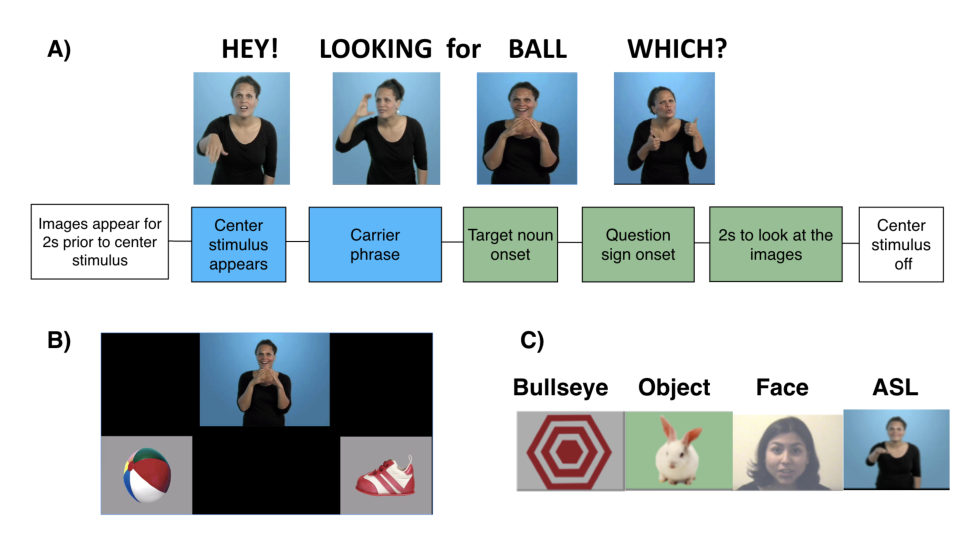
\includegraphics[width=0.7\linewidth]{figs/trio-stim-1} 

}

\caption{Stimuli for Experiment 1. Panel A shows the timecourse of the linguistic stimuli for a single trial. Panel B shows the layout of the fixation locations for all tasks: the center stimulus, the target, and the distracter. Panel C shows the four center stimulus items: a static geometric shape (Bullseye), a static image of a familiar object (Object), a person speaking (Face), and a person signing (ASL).}\label{fig:trio-stim}
\end{figure}

There are differences between ASL and English question structures.
However, all linguistic stimuli shared the same trial structure:
language to attract participants' attention followed by a sentence
containing a target noun.

\emph{ASL linguistic stimuli.} We recorded two sets of ASL stimuli,
using two valid ASL sentence structures for questions: 1)
Sentence-initial wh-phrase: \enquote{HEY! WHERE {[}target noun{]}?} and
2) Sentence-final wh-phrase: \enquote{HEY! {[}target noun{]} WHERE?} Two
female native ASL users recorded several tokens of each sentence in a
child-directed register. Before each sentence, the signer produced a
common attention-getting gesture. Mean sign length was 1.25 sec, ranging
from 0.69 sec to 1.98 sec.

\emph{English linguistic stimuli.} All three tasks (Object, Bullseye,
and Face) featured the same female speaker who used natural
child-directed speech and said: \enquote{Look! Where's the (target
word)?} The target words were: ball, banana, book, cookie, juice, and
shoe. For the Face task, a female native English speaker was
video-recorded as she looked straight ahead and said, \enquote{Look!
Where's the (target word)?} Mean word length was 0.79 sec, ranging from
0.60 sec to 0.94 sec.

\emph{ASL and English visual stimuli.} The image set consisted of
colorful digitized pictures of objects presented in fixed pairs with no
phonological overlap (ASL task: cat---bird, car---book, bear---doll,
ball---shoe; English tasks: book-shoe, juice-banana, cookie-ball). Side
of target picture was counterbalanced across trials.

\emph{Trial structure.} On each trial, the child saw two images of
familiar objects on the screen for two seconds before the center
stimulus appeared. This time allowed the child to visually explore both
images. Next, the target sentence -- which consisted of a carrier
phrase, target noun, and question sign -- was presented, followed by two
seconds without language to allow the child to respond to the signer's
sentence. The trial structure of the Face, Object, and Bullseye tasks
were highly similar: children were given two seconds to visually explore
the objects prior to the appearance of the center stimulus, then
processed a target sentence, and finally were given two seconds of
silence to generate a response to the target noun.

\hypertarget{design-and-procedure}{%
\subsubsection{Design and procedure}\label{design-and-procedure}}

Children sat on their caregiver's lap and viewed the task on a screen
while their gaze was recorded using a digital camcorder. On each trial,
children saw two images of familiar objects on the screen for two
seconds before the center stimulus appeared (see Figure 1). Then they
processed the target sentence -- which consisted of a carrier phrase, a
target noun, and a question -- followed by two seconds without language
to allow for a response. Participants saw 32 test trials with several
filler trials interspersed to maintain interest.

\emph{Coding.} Participants' gaze patterns were coded (33-ms resolution)
as being fixated on either the center stimulus, one of the images,
shifting between pictures, or away. To assess inter-coder reliability,
25\% of the videos were re-coded. Agreement was scored at the level of
individual frames of video and averaged 98\% on these reliability
assessments.

\hypertarget{results-and-discussion}{%
\subsection{Results and Discussion}\label{results-and-discussion}}

\begin{figure}[tb]

{\centering 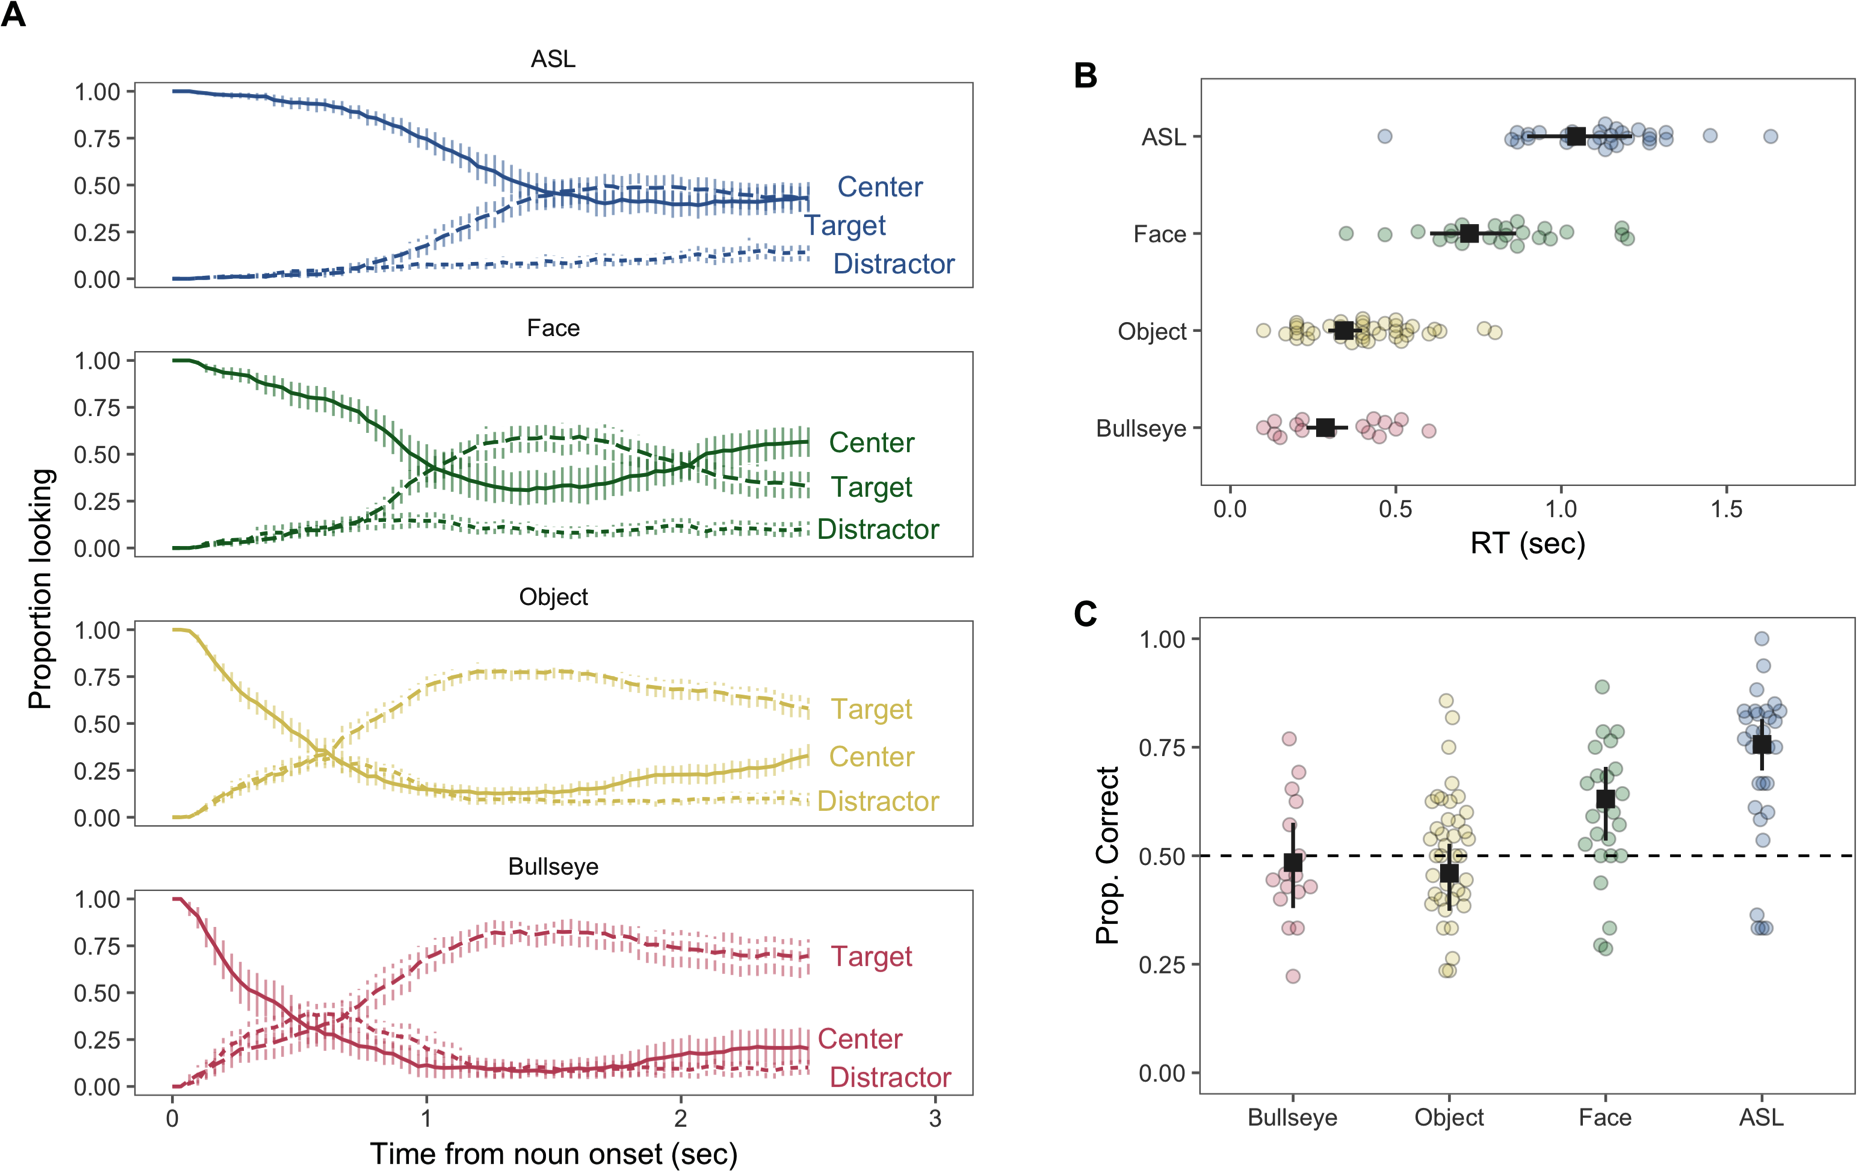
\includegraphics[width=0.9\linewidth]{figs/speed-acc-trio-plot-1} 

}

\caption{Timecourse looking, first shift Reaction Time (RT), and Accuracy results for children in Experiment 1. Panel A shows the overall looking to the center, target, and distracter stimulus for each context. Panel B shows the distribution of RTs for each participant. Each point represents a participant's average RT. Color represents the processing context. Panel C shows the same information but for first shift accuracy.}\label{fig:speed-acc-trio-plot}
\end{figure}

\hypertarget{behavioral-analyses}{%
\subsubsection{Behavioral analyses}\label{behavioral-analyses}}

\emph{RT.} Visual inspection of the Fig 2, panel A suggests that there
was a speed accuracy tradeoff in the ASL, Face, and Bullseye conditions,
with incorrect shifts tending to be faster than correct shifts. To
quantify differences across the groups, we fit a linear mixed-effects
regression predicting first shift RT as a function of center stimulus
type, controlling for age, and including user-defined contrasts to test
specific comparisons of interest:
\texttt{Log(RT) $\sim$ center stimulus type + age +  (1 | subject) + (1 | item)}.
We found that (a) ASL learners generated slower RTs compared to all of
the spoken English samples (\(\beta\) = -0.97, \(p\) \textless{} .001),
(b) ASL learners' shifts were slower compared directly to participants
in the Face task (\(\beta\) = -0.42, \(p\) \textless{} .001), and (c)
participants in the Face task shifted slower compared to participants in
the Object and Bullseye tasks (\(\beta\) = -0.73, \(p\) \textless{}
.001).

\emph{Accuracy.} Next we compared the accuracy of first shifts across
the different tasks by fitting a mixed-effects logistic regression with
the same specifications and contrasts as the RT model. We found that (a)
ASL learners were more accurate compared to all of the spoken English
samples (\(\beta\) = -0.78, \(p\) \textless{} .001), (b) ASL learners
were more accurate when directly compared to participants in the Face
task (\(\beta\) = -0.62, \(p\) = 0.001), and (c) participants in the
Face task were numerically more accurate compared to participants in the
Object and Bullseye tasks (\(\beta\) = -0.73) but this effect was not
significant (\(p\) = 0.089).

\hypertarget{model-based-analyses}{%
\subsubsection{Model-based analyses}\label{model-based-analyses}}

\begin{figure}[tb]

{\centering 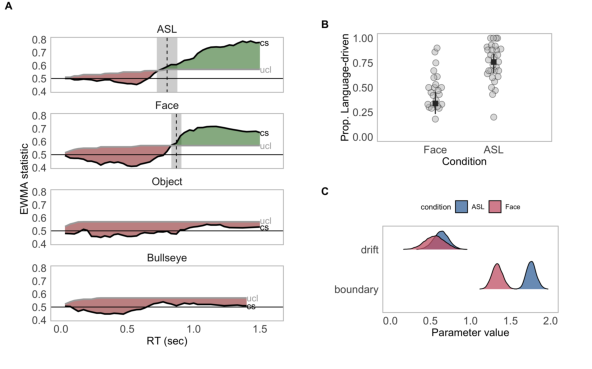
\includegraphics[width=0.9\linewidth]{figs/trio-model-plot-1} 

}

\caption{Results for the model-based analyses in Experiment 1. Panel A shows a control chart representing the timecourse of the EWMA statistic. The black curve represents the evolution of the control statistic (CS) as a function of reaction time. The grey curve represents the upper control limit (UCL). The vertical dashed line is the median cutoff value (point when the control process shifts out of a guessing state). The grey shaded area represents the 95\% confidence interval around the estimate of the median cutoff point, and the shaded ribbons represent the proportion of responses that were categorized as guesses (red) and language-driven (green). Panel B shows a summary of the proprotion of shifts that were categorized as language-driven for the Face and ASL tasks. Panel C shows the posterior distributions for the boundary and drift rate parameters for the Face and ASL tasks.}\label{fig:trio-model-plot}
\end{figure}

\emph{EWMA.} Figure 3 shows changes in the control statistic (CS) and
the upper control limit (UCL) as a function of participants' RTs. Each
CS starts at chance performance and below the UCL. In the ASL and Face
tasks, the CS value begins to increase with RTs around 0.7 seconds after
noun onset and eventually crosses the UCL, indicating that responses
\textgreater{} 0.7 sec were on average above chance levels. In contrast,
the CS in the Object and Bullseye tasks never crossed the UCL,
indicating that children's shifts were equally likely to land on the
target or the distracter, regardless of when they were initiated. This
result suggests that first shifts in the Bullseye/Object tasks were not
language-driven and may instead have reflected a different process such
as gathering more information about the referents in the visual world.

Next, we compared the EWMA output for participants in the ASL and Face
tasks. We found that ASL learners generated fewer shifts when the CS was
below the UCL (\(\beta\) = -1.65, \(p\) \textless{} .001), indicating
that a larger proportion of their initial shifts away were
language-driven (see the differences in the red shaded area in Fig 3).
We did not find evidence for a difference in the timing of when the CS
crossed the UCL (\(\beta\) = -0.04, \(p\) = 0.331), indicating that both
groups began to generate language-driven shifts about the same time
after noun onset.

\emph{HDDM.} Using the output of the EWMA, we compared the timing and
accuracy of language-driven shifts for participants in the ASL and Face
tasks.\footnote{We report the mean and the 95\% highest density interval
  (HDI) of the posterior distributions for each parameter. The HDI
  represents the range of credible values given the model specification
  and the data. We chose not to interpret the DDM fits for the
  Bullseye/Face tasks since there was no suggestion of any non-guessing
  signal.} We found that ASL learners had a higher estimate for the
boundary separation parameter compared to the Face participants (ASL
boundary = 1.76, HDI = {[}1.65, 1.88{]}; Face boundary = 1.34, HDI =
{[}1.21, 1.47{]}), with no overlap in the credible values (see Fig 4).
This suggests that ASL learners accumulated more evidence about the
linguistic signal before generating an eye movement. We found high
overlap for estimates of the drift rate parameter, indicating that both
groups processed the linguistic information with similar efficiency (ASL
drift = 0.63, HDI = {[}0.44, 0.82{]}; Face drift = 0.55, HDI = {[}0.30,
0.80{]}).

Taken together, the behavioral analyses and the EWMA/HDDM results
provide converging support that ASL learners were sensitive to the value
of delaying eye movements away from the language source. Compared to
spoken language learners, children learning ASL prioritized accuracy
over speed, produced fewer nonlanguage-driven shifts away from the
center stimulus, and were more accurate with these gaze shifts.
Importantly, we did not see evidence in the HDDM model fits that these
accuracy differences could be explained by differential rates of
information accumulation. Instead, the model-based analyses suggest that
ASL learners increased their decision threshold for generating a
response.

We hypothesized that this prioritization of gathering additional
information is an adaptive response to the channel competition present
when processing a visual-manual language. That is, when ASL learners
shift gaze away a signer, they are deciding to leave an area of the
visual world that provides a great deal of useful and interesting
information. Moreover, unlike children leanring spoken languages, ASL
learners cannot gather more of the linguistic signal while looking at
the objects. Thus, an adaptive language comprehension system would
increase levels of certainty before generating a response to maintain
robust understanding.

It is important to point out that these findings are based on
exploratory analyses, and our information seeking account was developed
to account for these differences. There are, however, several,
potentially important differences between the stimuli, apparatus, and
populations that limit the sterngth of our interpretation of these data
and the generality of our account. Thus, in Experiment 2, we set out to
perform a well-controlled, confirmatory test of our adaptive information
seeking account of eye movements during grounded language comprehension.

\hypertarget{experiment-2}{%
\section{Experiment 2}\label{experiment-2}}

In Experiment 2, we attempt to replicate a key finding from Experiment
1: that increasing the competition between fixating the language source
and the nonlinguistic visual world reduces nonlanguage-driven eye
movements. Moreover, we conducted a confirmatory test of our hypothesis
that also controlled for the population differences present in
Experiment 1. We tested a sample of English-speaking adults using a
within-participants manipulation of the center stimulus type. We used
the Face and Bullseye stimulus sets from Experiment 1 and added two new
conditions: Text, where the verbal language information was accompanied
by a word-by-word display of printed text (see Fig 1), and
Text-no-audio, where the spoken language stimulus was removed. We chose
text processing since, like sign language comprehension, the linguistic
information is gathered via fixations to the visual world.

Our key behavioral prediction is that participants in the Text
conditions should produce a higher proportion of language-driven shifts
as indexed by the EWMA model output. We did not have strong predictions
for the DDM parameter fits since the goal of the Text manipulation was
to modulate participants' strategic allocation of visual attention and
not the accuracy/efficiency of information processing.

\hypertarget{methods-1}{%
\subsection{Methods}\label{methods-1}}

\hypertarget{participants-1}{%
\subsubsection{Participants}\label{participants-1}}

25 Stanford undergraduates participated (5 male) for course credit. All
participants were monolingual, native English speakers and had normal
vision.

\hypertarget{stimuli-1}{%
\subsubsection{Stimuli}\label{stimuli-1}}

Audio and visual stimuli were identical to the Face and Bullseye tasks
in Experiment 1. We included a new center fixation stimulus type:
printed text. The text was displayed in a white font on a black
background and was programmed such that only a single word appeared on
the screen, with each word appearing for the same duration as the
corresponding word in the spoken language stimuli.

\hypertarget{design-and-procedure-1}{%
\subsubsection{Design and procedure}\label{design-and-procedure-1}}

The design was nearly identical to Experiment 1, with the exception of a
change to a within-subjects manipulation where each participant
completed all four tasks (Bullseye, Face, Text, and Text-no-audio). In
the Text condition, spoken language accompanied the printed text. In the
Text-no-audio condition, the spoken language stimulus was removed.
Participants saw a total of 128 trials while their eye movements were
tracked using automated eye-tracking software.

\hypertarget{results-and-discussion-1}{%
\subsection{Results and Discussion}\label{results-and-discussion-1}}

\begin{figure}[tb]

{\centering 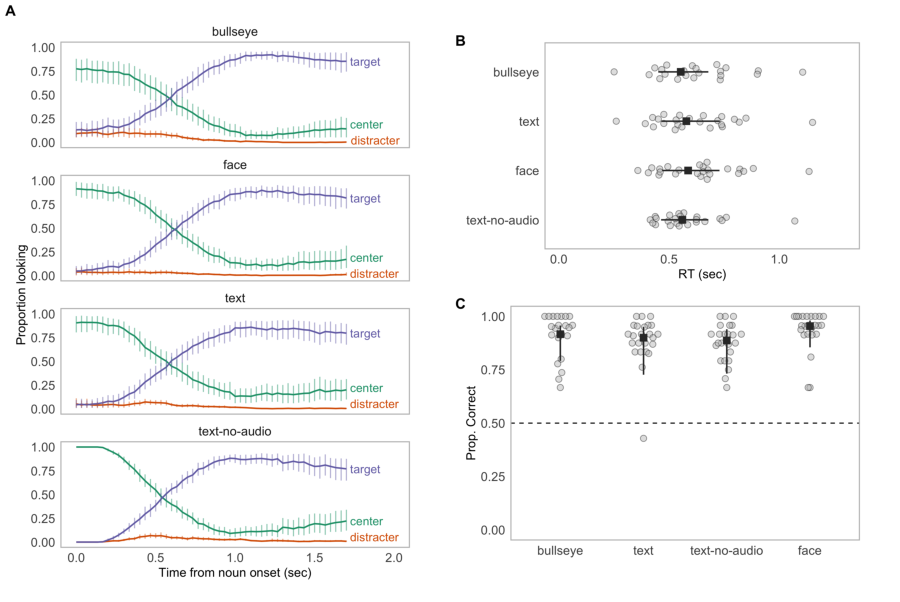
\includegraphics[width=0.85\linewidth]{figs/text-plot-1} 

}

\caption{Results for the model-based analyses in Experiment 2. All plotting conventions are the same as in Figure 2.}\label{fig:text-plot}
\end{figure}

\hypertarget{behavioral-analyses-1}{%
\subsubsection{Behavioral analyses}\label{behavioral-analyses-1}}

\emph{RT.} Visual inspection of Figure 5, panel A suggests that there
was a speed-accuracy tradeoff for all conditions: incorrect gaze shifts
tended to be faster than correct shifts. We fit a linear mixed-effects
regression with the same specification as in Experiment 1, but we added
by-subject intercepts and slopes for each center stimulus type to
account for our within-subjects manipulation. We did not find evidence
that RTs were different across conditions (all \(p\) \textgreater{}
.05).

\emph{Accuracy.} Next, we modeled accuracy using a mixed-effects
logistic regression with the same specifications (see Panel B of Fig 5).
We found that adults' first shifts were highly accurate, and, in
contrast to the children in Experiment 1, their responses were above
chance level even in the Bullseye condition when the center stimulus was
not salient or informative. We also found that participants tended to be
less accurate in the Text conditions compared to conditions without text
(\(\beta\) = 1.18, \(p\) = 0.00). We did find not any other
statistically significant differences.

\hypertarget{model-based-analyses-1}{%
\subsubsection{Model-based analyses}\label{model-based-analyses-1}}

\begin{figure}[tb]

{\centering 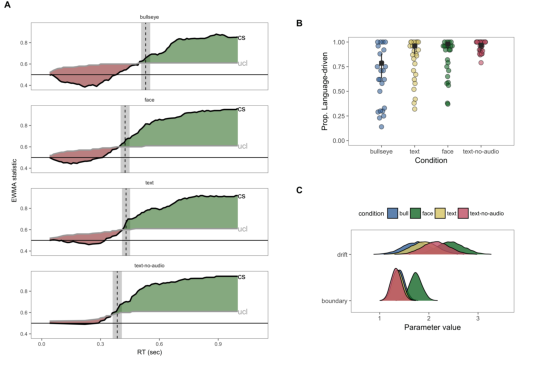
\includegraphics[width=0.9\linewidth]{figs/text-model-plots-1} 

}

\caption{Results for the model-based analyses of Experiment 2. All plotting conventions are the same as Figure 3.}\label{fig:text-model-plots}
\end{figure}

\emph{EWMA.} For all four conditions, the CS crossed the UCL (see Fig
6), suggesting that for all tasks some proportion of adults' shifts were
language-driven. Interestingly, we found a graded effect of condition
(see the shift in the vertical dashed lines in Fig 5) on the point when
the CS crossed the UCL such that the Text-no-audio condition occurred
earliest (\(M_{text-no-audio}\) = 0.39), followed by the Text and Face
conditions that were not different from one another (\(M_{text}\) =
0.44, \(M_{face}\) = 0.45, \(p\) \textgreater{} .05), and finally the
Bullseye condition (\(M_{bullseye}\) = 0.54). We also found the same
graded difference in the proportion of shifts that occurred while the CS
was below the UCL (see the red vs.~green shaded area in Fig 5),
indicating a higher proportion of first shifts were language-driven in
the Text conditions, with the highest proportion in the Text-no-audio
condition when tested against the three other conditions
(\(M_{text-no-audio}\) = 3.79, \(\beta\) = 1.74, \(p\) \textless{}
.001). These results provide strong evidence for our key prediction:
that increasing the value of fixating the language source reduces
exploratory gaze shifts to the nonlinguistic visual world.

\emph{HDDM.} Using the output of the EWMA, we fit the same HDDM as in
Experiment 1. There was high overlap of the posterior distributions for
the drift rate parameters (see Fig 4, panel B), suggesting that
participants gathered the linguistic information with similar
efficiency. We also found high overlap in the distribution of credible
boundary separation estimates for the Bullseye, Text, and Text-no-audio
conditions. Interestingly, we found some evidence for a higher boundary
separation in the Face condition compared to the other three center
stimulus types (Face boundary = 1.73, HDI = {[}1.49, 1.98{]}; Bullseye
boundary = 1.40, HDI = {[}1.19, 1.62{]}; Text boundary = 1.37, HDI =
{[}1.16, 1.58{]}; Text-no-audio boundary = 1.34, HDI = {[}1.14,
1.55{]}), suggesting that adults higher accuracy in this condition was
driven by accumulating more information before generating a response.

Together, these results suggest that adults were sensitive to the
tradeoff between gathering different kinds of information. When
processing text, people generated fewer nonlanguage-driven shifts (EWMA
results) but their processing efficiency of the linguistic signal itself
did not change (HDDM results). Interestingly, we found a graded
difference in the EWMA results between the Text and Text-no-audio
conditions, with the lowest proportion of early, nonlanguage-driven
shifts occurring while processing text without the verbal stimuli. This
behavior makes sense; if the adults could rely on the auditory channel
to gather the linguistic information, then the value of fixating the
text display decreases. In contrast to the children in Experiment 1,
adults were highly accurate in the Bullseye condition, perhaps because
they construed the Bullseye as a center fixation that they \emph{should}
fixate, or perhaps they had better encoded the location/identity of the
two referents prior to the start of the target sentence.

\hypertarget{experiment-3}{%
\section{Experiment 3}\label{experiment-3}}

In this experiment, we recorded adults and children's eye movements
during a real-time language comprehension task where participants
processed familiar sentences (e.g., \enquote{Where's the ball?}) while
looking at a simplified visual world with three fixation targets (see
Fig.~\ref{fig:stimuli_plot}). Using a within-participants design, we
manipulated the signal-to-noise ratio of the auditory signal by
convolving the acoustic input with brown noise (random noise with
greater energy at lower frequencies).

We predicted that processing speech in a noisy context would make
participants less likely to shift before collecting sufficient
information.\footnote{See \url{https://osf.io/g8h9r/} for a
  pre-registration of the analysis plan.} This delay, in turn, would
lead to a lower proportion of shifts flagged as random/exploratory in
the EWMA analysis, and a pattern of DDM results indicating a
prioritization of accuracy over and above speed of responding (see the
Analysis Plan section below for more details on the models). We also
predicted a developmental difference -- that children would produce a
higher proportion of random shifts and accumulate information less
efficiently compared to adults; and a developmental parallel -- that
children would show the same pattern of adapting gaze patterns to gather
more visual information in the noisy processing context.

\hypertarget{methods-2}{%
\subsection{Methods}\label{methods-2}}

\hypertarget{participants-2}{%
\subsubsection{Participants}\label{participants-2}}

Participants were native, monolingual English-learning children (\(n=\)
39; 22 F) and adults (\(n=\) 31; 22 F). All participants had no reported
history of developmental or language delay and normal vision. 14
participants (11 children, 3 adults) were run but not included in the
analysis because either the eye tracker falied to calibrate (2 children,
3 adults) or the participant did not complete the task (9 children).

\hypertarget{stimuli-2}{%
\subsubsection{Stimuli}\label{stimuli-2}}

\emph{Linguistic stimuli.} The video/audio stimuli were recorded in a
sound-proof room and featured two female speakers who used natural
child-directed speech and said one of two phrases: \enquote{Hey! Can you
find the (target word)} or ``Look! Where's the (target word) -- see
panel A of Fig.~\ref{fig:stimuli_plot}. The target words were: ball,
bunny, boat, bottle, cookie, juice, chicken, and shoe. The target words
varied in length (shortest = 411.68 ms, longest = 779.62 ms) with an
average length of 586.71 ms.

\emph{Noise manipulation}. To create the stimuli in the noise condition,
we convolved each recording with Brown noise using the Audacity audio
editor. The average signal-to-noise ratio\footnote{The ratio of signal
  power to the noise power, with values greater than 0 dB indicating
  more signal than noise.} in the noise condition was 2.87 dB compared
to the clear condition, which was 35.05 dB.

\emph{Visual stimuli.} The image set consisted of colorful digitized
pictures of objects presented in fixed pairs with no phonological
overlap between the target and the distractor image (cookie-bottle,
boat-juice, bunny-chicken, shoe-ball). The side of the target picture
was counterbalanced across trials.

\hypertarget{design-and-procedure-2}{%
\subsubsection{Design and procedure}\label{design-and-procedure-2}}

Participants viewed the task on a screen while their gaze was tracked
using an SMI RED corneal-reflection eye-tracker mounted on an LCD
monitor, sampling at 60 Hz. The eye-tracker was first calibrated for
each participant using a 6-point calibration. On each trial,
participants saw two images of familiar objects on the screen for two
seconds before the center stimulus appeared (see
Fig.~\ref{fig:stimuli_plot}). Next, they processed the target sentence
-- which consisted of a carrier phrase, a target noun, and a question --
followed by two seconds without language to allow for a response. Child
participants saw 32 trials (16 noise trials; 16 clear trials) with
several filler trials interspersed to maintain interest. Adult
participants saw 64 trials (32 noise; 32 clear). The noise manipulation
was presented in a blocked design with the order of block
counterbalanced across participants.

\hypertarget{results-and-discussion-2}{%
\subsection{Results and discussion}\label{results-and-discussion-2}}

\hypertarget{behavioral-analyses-2}{%
\subsubsection{Behavioral analyses:}\label{behavioral-analyses-2}}

\begin{figure}[tb]

{\centering 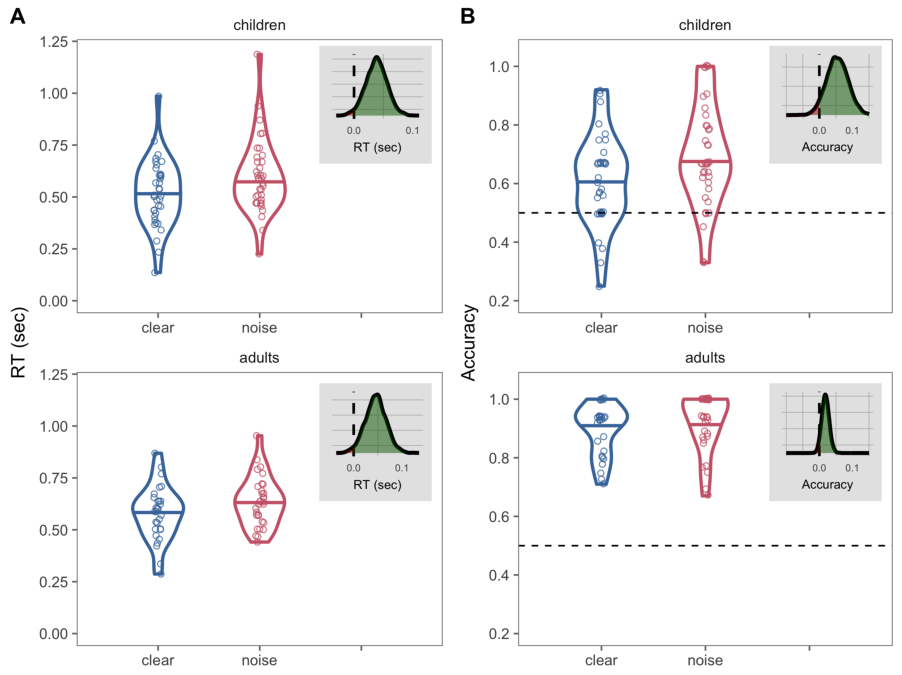
\includegraphics[width=0.8\linewidth]{figs/noise-acc-rt-1} 

}

\caption{Behavioral results for children and adults in Experiment 3. Panel A shows the overall looking to the center, target, and distracter stimulus for each processing condition and age group. Panel B shows the distribution of RTs for each participant and the pairwise contrast between the noise and clear conditions. The square point represents the mean value for each mesure. The vertical dashed line represents the null model of zero condition difference. The width each point represents the 95\% HDI. Panel C shows the same information but for first shift accuracy.}\label{fig:noise-acc-rt}
\end{figure}

\textbf{RT.} To make RTs more suitable for modeling on a linear scale,
we analyzed responses in log space with the final model specified as:
\texttt{$log(RT) \sim noise\_condition + age\_group + (noise\_condition \mid sub\_id ) + (noise\_condition \mid target\_item)$}.
Panel A of Fig.~\ref{fig:noise_acc_rt_noise_plot} shows the full RT data
distribution and the full posterior distribution of the estimated RT
difference between the noise and clear conditions. Both children and
adults were slower to identify the target in the noise condition
(Children \(M_{noise}\) = 500.19 ms; Adult \(M_{noise}\) = 595.23 ms),
as compared to the clear condition (Children \(M_{clear}\) = 455.72 ms;
Adult \(M_{clear}\) = 542.45 ms). RTs in the noise condition were 48.82
ms slower on average, with a 95\% HDI ranging from 3.72 ms to 96.26 ms,
and not including the null value of zero condition difference. Older
children responded faster than younger children (\(M_{age}\) = -0.44,
{[}-0.74, -0.16{]}), with little evidence for an interaction between age
and condition.

\textbf{Accuracy.} Next, we modeled adults and children's first shift
accuracy using a mixed-effects logistic regression with the same
specifications (see Panel B of Fig.~\ref{fig:noise_acc_rt_noise_plot}).
Both groups were more accurate than a model of random responding (null
value of \(0.5\) falling well outside the lower bound of the 95\% HDI
for all group means). Adults were more accurate (\(M_{adults} =\) 90\%)
than children (\(M_{children} =\) 61\%). The key result is that both
groups showed evidence of higher accuracy in the noise condition:
children (\(M_{noise}\) = 67\%; \(M_{clear}\) = 61\%) and adults
(\(M_{noise}\) = 92\%; \(M_{clear}\) = 90\%). Accuracy in the noise
condition was on average 4\% higher, with a 95\% HDI from -1\% to 12\%.
Note that the null value of zero difference falls at the very edge of
the HDI. But 95\% of the credible values are greater than zero,
providing evidence for higher accuracy in the noise condition. Within
the child sample, there was no evidence of a main effect of age or an
interaction between age and noise condition.

\hypertarget{model-based-analyses-2}{%
\subsubsection{Model-based analyses:}\label{model-based-analyses-2}}

\begin{figure}[tb]

{\centering 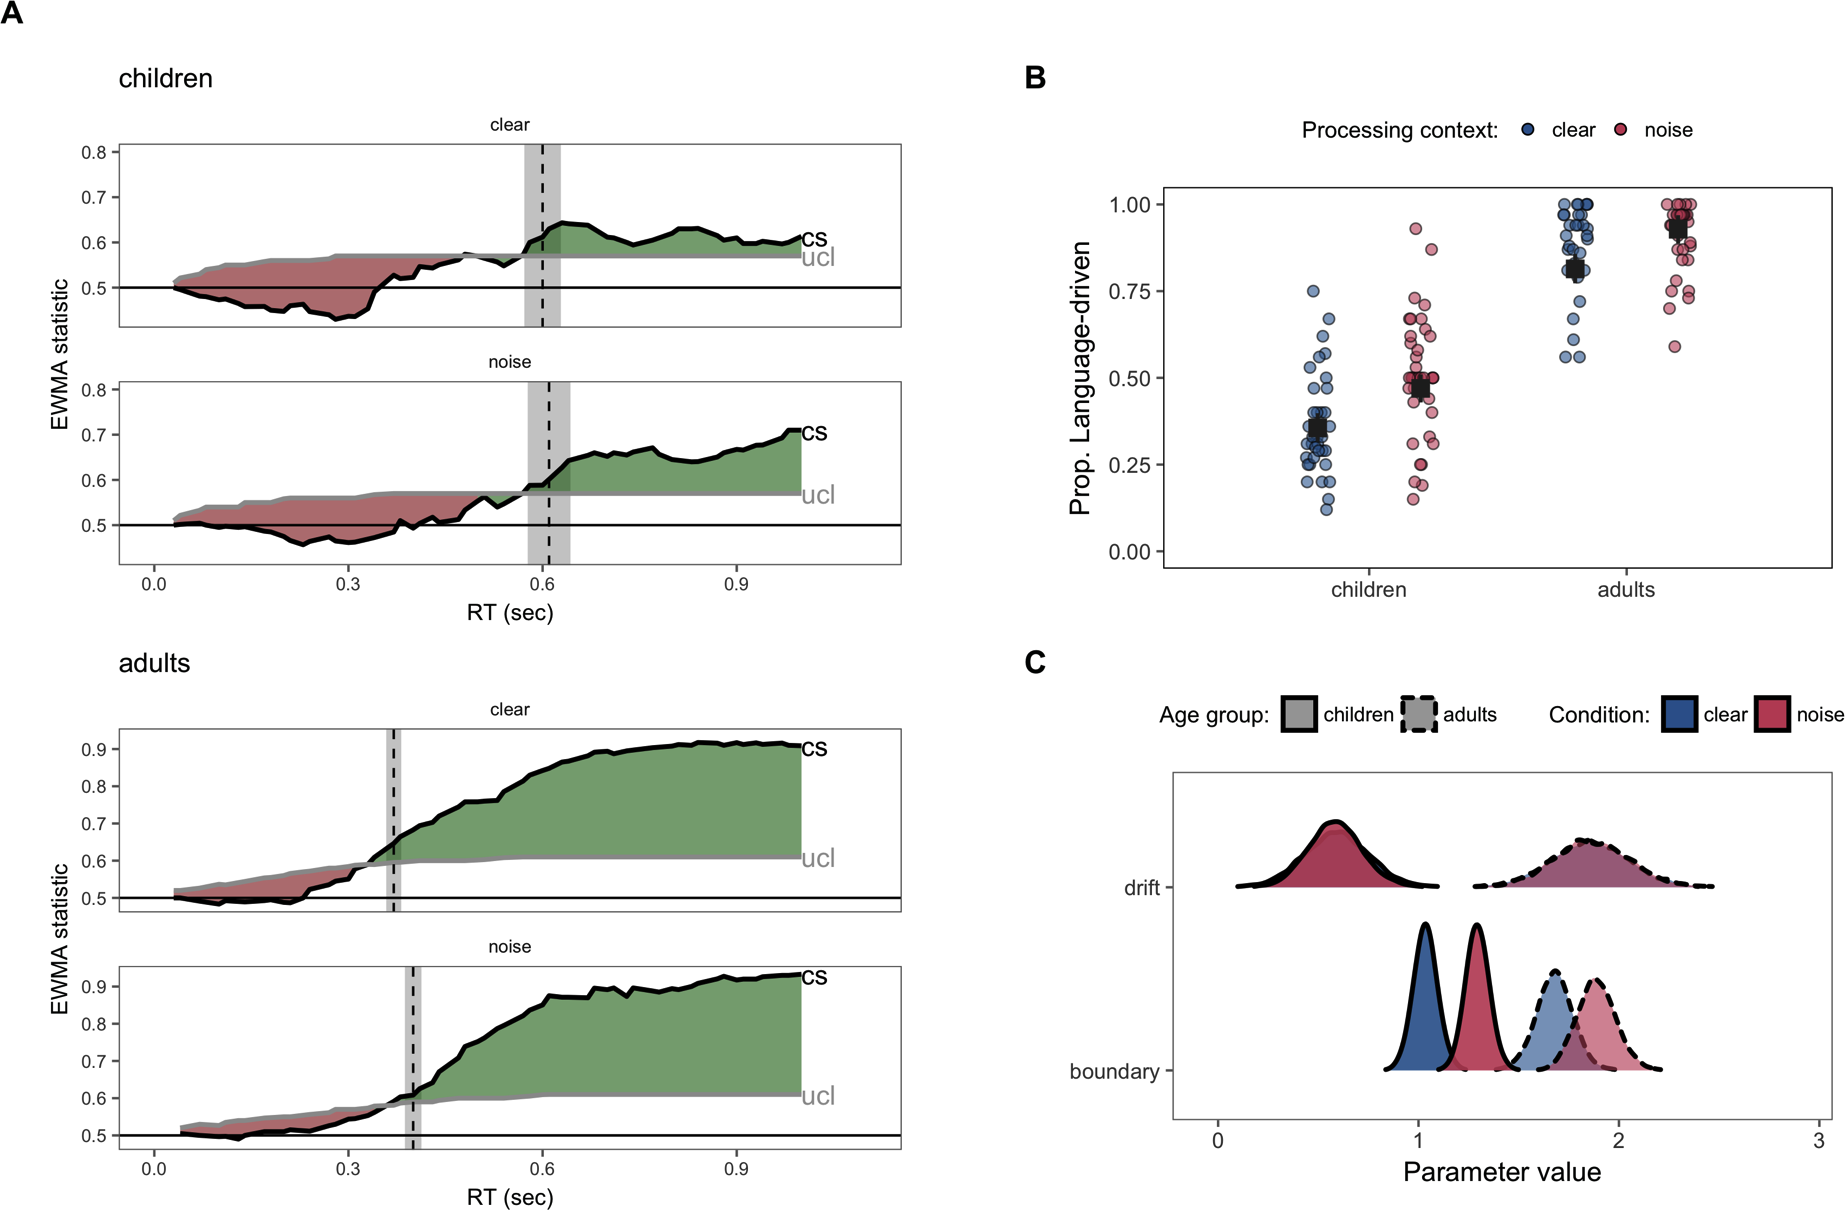
\includegraphics[width=0.9\linewidth]{figs/noise-model-plots-1} 

}

\caption{Results for the model-based analyses for Experiment 3. The majority of plotting conventions are the same as Figure 3. In Panel C, linetype and alpha value represent age group: children vs. adults.}\label{fig:noise-model-plots}
\end{figure}

\textbf{EWMA.} Fig.~\ref{fig:noise_ewma_violin_plot} shows the
proportion of shifts that the model classified as random
vs.~language-driven for each age group and processing context. On
average, 41\% (95\% HDI: 32\%, 50\%) of children's shifts were
categorized as language-driven, which was significantly fewer than
adults, 87\% (95\% HDI: 78\%, 96\%). Critically, processing speech in a
noisy context caused both adults and children to generate a higher
proportion of language-driven shifts (i.e., fewer random, exploratory
shifts away from the speaker), with the 95\% HDI excluding the null
value of zero condition difference (\(\beta_{noise}\) = 11\%, {[}7.00\%,
16\%{]}). Within the child sample, older children generated fewer
random, early shifts (\(M_{age}\) = -0.21, {[}-0.35, -0.08{]}). There
was no eivdence of an interaction between age and condition. This
pattern of results suggests that the noise condition caused participants
to increase visual fixations to the language source, leading them to
generate fewer exploratory, random shifts before accumulating sufficient
information to respond accurately.

\textbf{HDDM.} Fig.~\ref{fig:hddm_plot_noise} shows the full posterior
distributions for the HDDM output. Children had lower drift rates
(children \(M_{drift}\) = NA; adults \(M_{drift}\) = NA) and boundary
separation estimates (children \(M_{boundary}\) = 1.02; adults
\(M_{boundary}\) = 1.33) as compared to adults, suggesting that children
were less efficient and less cautious in their responding. The noise
manipulation selectively affected the boundary separation parameter,
with higher estimates in the noise condition for both age groups
(\(\beta_{noise}\) = 0.26, {[}0.10, 0.42{]}). This result suggests that
participants' in the noise condition prioritized information
accumulation over speed when generating an eye movement in response to
the incoming language. This increased decision threshold led to higher
accuracy. Moreover, the high overlap in estimates of drift rate suggests
that participants were able to integrate the visual and auditory signals
such that they could achieve a level of processing efficiency comparable
to the clear processing context.

Taken together, the behavioral and EWMA/HDDM results provide converging
support for the predictions of our information-seeking account.
Processing speech in noise caused listeners to seek additional visual
information to support language comprehension. Moreover, we observed a
very similar pattern of behavior in children and adults, with both
groups producing more language-driven shifts and prioritizing accuracy
over speed in the more challenging, noisy environment.

\hypertarget{general-discussion}{%
\section{General Discussion}\label{general-discussion}}

Language comprehension in grounded contexts involves integrating
information from the visual and linguistic signals. But the value of
integrating visual information depends on the processing context. Here,
we presented a test of an information-seeking account of eye movements
during language processing: that listeners flexibly adapt gaze patterns
in response to the value of seeking visual information for accurate
language understanding. We showed that children and adults generate
slower but more accurate gaze shifts away from a speaker when processing
speech in a noisy context. Both groups showed evidence of prioritizing
information accumulation over speed (HDDM) while guessing less often
(EWMA). Listeners were able to achieve higher accuracy in the more
challenging, noisy context. Together, these results suggest that in
settings with a degraded linguistic signal, listeners support language
comprehension by seeking additional language-relevant information from
the visual world.

These results synthesize ideas from several research programs, including
work on language-mediated visual attention (Tanenhaus et al., 1995),
goal-based accounts of vision during everyday tasks (Hayhoe \& Ballard,
2005), and work on effortful listening (Van Engen \& Peelle, 2014).
Moreover, our findings parallel recent work by McMurray, Farris-Trimble,
and Rigler (2017) showing that individuals with Cochlear Implants, who
are consistently processing degraded auditory input, are more likely to
delay the process of lexical access as measured by slower gaze shifts to
named referents and fewer incorrect gaze shifts to phonological onset
competitors. McMurray et al. (2017) also found that they could replicate
these changes to gaze patterns in adults with typical hearing by
degrading the auditory stimuli so that it shared features with the
output of a cochlear implant (noise-vocoded speech).

The results reported here also dovetail with recent developmental work
by Yurovsky et al. (2017). In that study, preschoolers, like adults,
were able to integrate top-down expectations about the kinds of things
speakers are likely to talk about with bottom-up cues from auditory
perception. Yurovsky et al. (2017) situated this finding within the
framework of modeling language as a \emph{noisy channel} where listeners
combine expectations with perceptual data and weight each based on its
reliability. Here, we found a similar developmental parallel in language
processing: that 3-5 year-olds, like adults, adapted their gaze patterns
to seek additional visual information when the auditory signal became
less reliable. This adaptation allowed listeners to generate more
accurate responses in the more challenging, noisy context.

\hypertarget{limitations}{%
\subsection{Limitations}\label{limitations}}

This work has several important limitations that pave the way for future
work. First, we chose to focus on a single decision about visual
fixation to provide a window onto the dynamics of decision-making across
different language processing contexts. But our analysis does not
consider the rich information present in the gaze patterns that occur
leading up to this decision. In our future work, we aim to measure how
changes in the language environment might lead to shifts in the dynamics
of gaze across a wider timescale. For example, perhaps listeners gather
more information about the objects in the scene before the sentence in
anticipation of allocating more attention to the speaker once they start
to speak. Second, we chose one instantiation of a noisy processing
context -- random background noise. But we think our findings should
generalize to contexts where other kinds of noise -- e.g., uncertainty
over a speaker's reliability or when processing accented speech -- make
gathering visual information from the speaker more useful for language
understanding.

\hypertarget{conclusion}{%
\subsection{Conclusion}\label{conclusion}}

This experiment tested the generalizability of our information-seeking
account of eye movements within the domain of grounded language
comprehension. But the account could be applied to the language
acquisition context. Consider that early in language learning, children
are acquiring novel word-object links while also learning about visual
object categories. Both of these tasks produce different goals that
should, in turn, modulate children's decisions about where to allocate
visual attention -- e.g., seeking nonlinguistic cues to reference such
as eye gaze and pointing become critical when you are unfamiliar with
the information in the linguistic signal. More generally, this work
integrates goal-based models of eye-movements with language
comprehension in grounded, social contexts. This approach presents a way
forward for explaining fixation behaviors across a wider variety
processing contexts and during different stages of language learning.

\newpage

\hypertarget{references}{%
\section{References}\label{references}}

\setlength{\parindent}{-0.5in}
\setlength{\leftskip}{0.5in}

\hypertarget{refs}{}
\leavevmode\hypertarget{ref-allopenna1998tracking}{}%
Allopenna, P. D., Magnuson, J. S., \& Tanenhaus, M. K. (1998). Tracking
the time course of spoken word recognition using eye movements: Evidence
for continuous mapping models. \emph{Journal of Memory and Language},
\emph{38}(4), 419--439.

\leavevmode\hypertarget{ref-altmann2007real}{}%
Altmann, G., \& Kamide, Y. (2007). The real-time mediation of visual
attention by language and world knowledge: Linking anticipatory (and
other) eye movements to linguistic processing. \emph{Journal of Memory
and Language}, \emph{57}(4), 502--518.

\leavevmode\hypertarget{ref-byers2017bilingual}{}%
Byers-Heinlein, K., Morin-Lessard, E., \& Lew-Williams, C. (2017).
Bilingual infants control their languages as they listen.
\emph{Proceedings of the National Academy of Sciences}, \emph{114}(34),
9032--9037.

\leavevmode\hypertarget{ref-dahan2005looking}{}%
Dahan, D., \& Tanenhaus, M. K. (2005). Looking at the rope when looking
for the snake: Conceptually mediated eye movements during spoken-word
recognition. \emph{Psychonomic Bulletin \& Review}, \emph{12}(3),
453--459.

\leavevmode\hypertarget{ref-erber1969interaction}{}%
Erber, N. P. (1969). Interaction of audition and vision in the
recognition of oral speech stimuli. \emph{Journal of Speech and Hearing
Research}, \emph{12}(2), 423--425.

\leavevmode\hypertarget{ref-fernald2006picking}{}%
Fernald, A., Perfors, A., \& Marchman, V. A. (2006). Picking up speed in
understanding: Speech processing efficiency and vocabulary growth across
the 2nd year. \emph{Developmental Psychology}, \emph{42}(1), 98.

\leavevmode\hypertarget{ref-fernald2008looking}{}%
Fernald, A., Zangl, R., Portillo, A. L., \& Marchman, V. A. (2008).
Looking while listening: Using eye movements to monitor spoken language.
\emph{Developmental Psycholinguistics: On-Line Methods in Children's
Language Processing}, \emph{44}, 97.

\leavevmode\hypertarget{ref-gabry2016rstanarm}{}%
Gabry, J., \& Goodrich, B. (2016). Rstanarm: Bayesian applied regression
modeling via stan. R package version 2.10. 0.

\leavevmode\hypertarget{ref-gold2000representation}{}%
Gold, J. I., \& Shadlen, M. N. (2000). Representation of a perceptual
decision in developing oculomotor commands. \emph{Nature},
\emph{404}(6776), 390.

\leavevmode\hypertarget{ref-hayhoe2005eye}{}%
Hayhoe, M., \& Ballard, D. (2005). Eye movements in natural behavior.
\emph{Trends in Cognitive Sciences}, \emph{9}(4), 188--194.

\leavevmode\hypertarget{ref-huettig2005word}{}%
Huettig, F., \& Altmann, G. T. (2005). Word meaning and the control of
eye fixation: Semantic competitor effects and the visual world paradigm.
\emph{Cognition}, \emph{96}(1), B23--B32.

\leavevmode\hypertarget{ref-macdonald1978visual}{}%
MacDonald, J., \& McGurk, H. (1978). Visual influences on speech
perception processes. \emph{Attention, Perception, \& Psychophysics},
\emph{24}(3), 253--257.

\leavevmode\hypertarget{ref-macdonald2018real}{}%
MacDonald, K., LaMarr, T., Corina, D., Marchman, V. A., \& Fernald, A.
(2018). Real-time lexical comprehension in young children learning
american sign language. \emph{Developmental Science}, e12672.

\leavevmode\hypertarget{ref-macdonald2006constraint}{}%
MacDonald, M. C., \& Seidenberg, M. S. (2006). Constraint satisfaction
accounts of lexical and sentence comprehension. \emph{Handbook of
Psycholinguistics}, \emph{2}, 581--611.

\leavevmode\hypertarget{ref-marchman2008speed}{}%
Marchman, V. A., \& Fernald, A. (2008). Speed of word recognition and
vocabulary knowledge in infancy predict cognitive and language outcomes
in later childhood. \emph{Developmental Science}, \emph{11}(3).

\leavevmode\hypertarget{ref-mcclelland1986trace}{}%
McClelland, J. L., \& Elman, J. L. (1986). The trace model of speech
perception. \emph{Cognitive Psychology}, \emph{18}(1), 1--86.

\leavevmode\hypertarget{ref-mcclelland2006there}{}%
McClelland, J. L., Mirman, D., \& Holt, L. L. (2006). Are there
interactive processes in speech perception? \emph{Trends in Cognitive
Sciences}, \emph{10}(8), 363--369.

\leavevmode\hypertarget{ref-mcmurray2017waiting}{}%
McMurray, B., Farris-Trimble, A., \& Rigler, H. (2017). Waiting for
lexical access: Cochlear implants or severely degraded input lead
listeners to process speech less incrementally. \emph{Cognition},
\emph{169}, 147--164.

\leavevmode\hypertarget{ref-nelson2007probabilistic}{}%
Nelson, J. D., \& Cottrell, G. W. (2007). A probabilistic model of eye
movements in concept formation. \emph{Neurocomputing}, \emph{70}(13-15),
2256--2272.

\leavevmode\hypertarget{ref-ratcliff2015individual}{}%
Ratcliff, R., \& Childers, R. (2015). Individual differences and fitting
methods for the two-choice diffusion model of decision making.
\emph{Decision}, \emph{2}(4), 237--279.

\leavevmode\hypertarget{ref-rigler2015slow}{}%
Rigler, H., Farris-Trimble, A., Greiner, L., Walker, J., Tomblin, J. B.,
\& McMurray, B. (2015). The slow developmental time course of real-time
spoken word recognition. \emph{Developmental Psychology}, \emph{51}(12),
1690.

\leavevmode\hypertarget{ref-salverda2011goal}{}%
Salverda, A. P., Brown, M., \& Tanenhaus, M. K. (2011). A goal-based
perspective on eye movements in visual world studies. \emph{Acta
Psychologica}, \emph{137}(2), 172--180.

\leavevmode\hypertarget{ref-schwartz2013language}{}%
Schwartz, R. G., Steinman, S., Ying, E., Mystal, E. Y., \& Houston, D.
M. (2013). Language processing in children with cochlear implants: A
preliminary report on lexical access for production and comprehension.
\emph{Clinical Linguistics \& Phonetics}, \emph{27}(4), 264--277.

\leavevmode\hypertarget{ref-spivey2002eye}{}%
Spivey, M. J., Tanenhaus, M. K., Eberhard, K. M., \& Sedivy, J. C.
(2002). Eye movements and spoken language comprehension: Effects of
visual context on syntactic ambiguity resolution. \emph{Cognitive
Psychology}, \emph{45}(4), 447--481.

\leavevmode\hypertarget{ref-tanenhaus1995integration}{}%
Tanenhaus, M. K., Spivey-Knowlton, M. J., Eberhard, K. M., \& Sedivy, J.
C. (1995). Integration of visual and linguistic information in spoken
language comprehension. \emph{Science}, \emph{268}(5217), 1632.

\leavevmode\hypertarget{ref-vandekerckhove2007fitting}{}%
Vandekerckhove, J., \& Tuerlinckx, F. (2007). Fitting the ratcliff
diffusion model to experimental data. \emph{Psychonomic Bulletin \&
Review}, \emph{14}(6), 1011--1026.

\leavevmode\hypertarget{ref-van2014listening}{}%
Van Engen, K. J., \& Peelle, J. E. (2014). Listening effort and accented
speech. \emph{Frontiers in Human Neuroscience}, \emph{8}.

\leavevmode\hypertarget{ref-venker2013individual}{}%
Venker, C. E., Eernisse, E. R., Saffran, J. R., \& Weismer, S. E.
(2013). Individual differences in the real-time comprehension of
children with asd. \emph{Autism Research}, \emph{6}(5), 417--432.

\leavevmode\hypertarget{ref-wiecki2013hddm}{}%
Wiecki, T. V., Sofer, I., \& Frank, M. J. (2013). HDDM: Hierarchical
bayesian estimation of the drift-diffusion model in python.
\emph{Frontiers in Neuroinformatics}, \emph{7}, 14.

\leavevmode\hypertarget{ref-yee2006eye}{}%
Yee, E., \& Sedivy, J. C. (2006). Eye movements to pictures reveal
transient semantic activation during spoken word recognition.
\emph{Journal of Experimental Psychology: Learning, Memory, and
Cognition}, \emph{32}(1), 1.

\leavevmode\hypertarget{ref-yurovsky2017preschoolers}{}%
Yurovsky, D., Case, S., \& Frank, M. C. (2017). Preschoolers flexibly
adapt to linguistic input in a noisy channel. \emph{Psychological
Science}, \emph{28}(1), 132--140.






\end{document}
